\chapter{Implementacija i korisničko sučelje}
		
		\section{Korištene tehnologije i alati}
		
			Komunikacija u timu realizirana je korištenjem aplikacija \underline{WhatsApp}\footnote{https://www.whatsapp.com/} i \underline{Discord} \footnote{https://discord.com/}. Za izradu	UML dijagrama korišten je alat \underline{Astah UML} \footnote{https://astah.net/products/astah-uml/}  , a kao sustav za upravljanje izvornim kodom \underline{Git}\footnote{https://git-scm.com/}. Udaljeni repozitorij projekta je dostupan na web platformi \underline{GitLab} \footnote{https://gitlab.com/} .
			Kao razvojno okruženje korišten je \underline{Visual Studio Code}\footnote{https://code.visualstudio.com/}. Prvenstveno se koristi kao uređivač teksta pri razvoju računalnih programa za operacijski sustav Windows, kao i za web-stranice, web-aplikacije, web-usluge i mobilne aplikacije. Aplikacija je napisana koristeći radni okvir \underline{Flask}\footnote{https://flask.palletsprojects.com/en/2.0.x/} i web poslužitelj \underline{Gunicorn}\footnote{https://gunicorn.org/} u jeziku \underline{Python 3.8}. \footnote{https://www.python.org/} za izradu backenda. Za izradu frontenda su se koristili razvojni okvir \underline{React}\footnote{https://reactjs.org/} i jezik \underline{JavaScript}\footnote{https://www.javascript.com/}. React, takoder poznat kao React.js ili ReactJS, je biblioteka u JavaScriptu za izgradnju korisničkih sučelja. React se najčešće koristi kao osnova	u razvoju web ili mobilnih aplikacija. Složene aplikacije u Reactu obično zahtijevaju korištenje dodatnih biblioteka za interakciju s API-jem. Web poslužitelj Gunicorn nadograđuje radni okvir Flask kako bi mogao posluživati više zahtjeva u isto vrijeme. Naša cijela infrastruktura se nalazi u oblaku na privatnom VPS poslužitelju, poslužuje zahtjeve pomoću \underline{NGINX}\footnote{https://nginx.org/en/} web poslužitelja na linux  ubuntu sustavu.
			Mrežna potpora našoj arhitekturi je \underline{CloudFlare} \footnote{https://www.cloudflare.com/} koja nam nudi usluge poput predmemorije (engl. cache) i DDoS zaštite. Bitan dio naše infrastrukture je baza podataka realizirana kroz \underline{PostgreSQL RDBMS}\footnote{https://www.postgresql.org/}.
			
			
			\eject 
		
	
		\section{Ispitivanje programskog rješenja}
		
			 Svi testovi izvršeni su pomoću skripte u Pythonu koristeći Selenium WebDriver i pytest. Ispitivanje se radilo po obrascima uporabe kako bi se provjerila osnovna funkcionalnost sustava, ali i nasumičnim kretanjima po aplikaciji kako bi se pronašle neočekivane greške(”bugovi”) ili nepredviđena ponašanja. Svaki dio sustava je ispitan, no zbog jednostavnosti u dokumentaciji će biti prikazan samo dio ispitivanja.
	
			
			\subsection{Ispitivanje komponenti}
			\textbf{Ispitni slučajevi}: \newline
			Provedeno je ispitivanje jedinca za 6 ispitnih slučajeva. Ti su slučajevi redom:
			\begin{enumerate}
				\item Konekcija na bazu podataka
				\item Provjera postojanja korisnika
				\item Dohvaćanje imena klase natjecanja
				\item Dohvaćanje zadatka
				\item Dohvaćanje imena zadatka
				\item Dohvaćanje virtualnog natjecanja
			\end{enumerate}
			
			\noindent  \textbf{Očekivani rezultati}: 
			\begin{enumerate}
				\item Uspješna spajanje s bazom podataka
				\item Uspješno/Neuspješno postojanje korisnika ovisno o parametrima
				\item Uspješno dohvaćanje imena klase natjecanja
				\item Uspješno dohvaćanje zadatka
				\item Uspješno dohvaćanje punog imena zadatka
				\item Uspješno dohvaćanje virtualnog natjecanja
			\end{enumerate}
			
			\begin{figure}[H]
				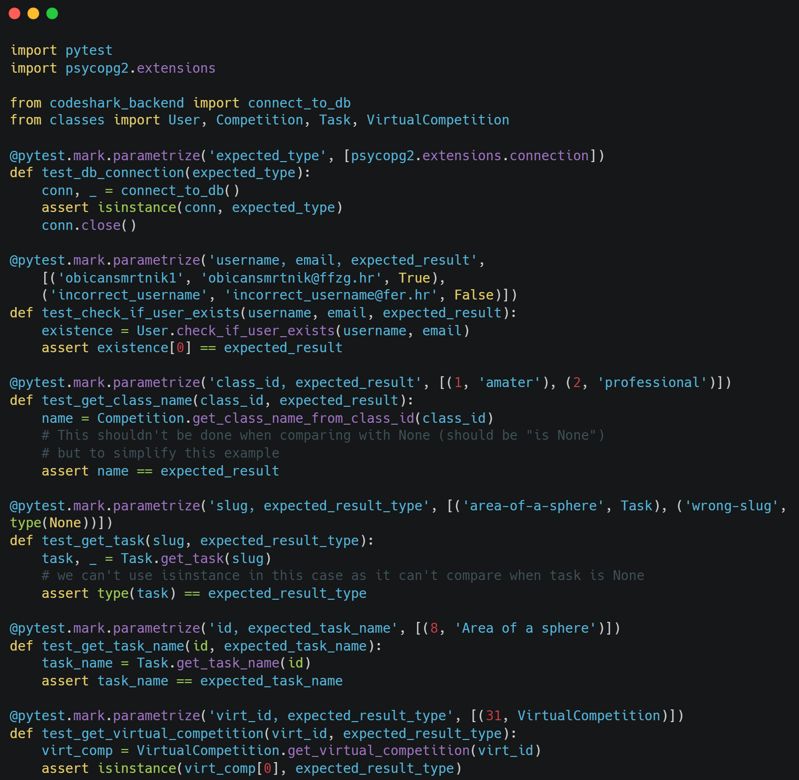
\includegraphics[width=\textwidth]{slike/IspitivanjeKomponenti.png} %veličina u odnosu na širinu linije
				\caption{Ispitivanje komponenti}
				\label{fig:IspitivanjeKomponenti} %label mora biti drugaciji za svaku sliku
			\end{figure}
		
			\begin{figure}[H]
				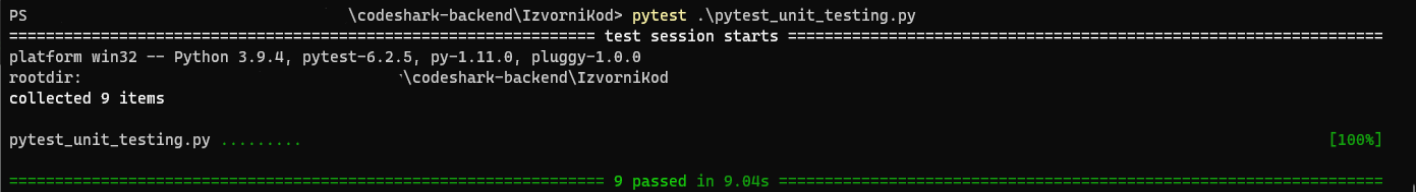
\includegraphics[width=\textwidth]{slike/IspitivanjeKomponentiRez.png} %veličina u odnosu na širinu linije
				\caption{Rezultat ispitivanja komponenti}
				\label{fig:IspitivanjeKomponentiRez} %label mora biti drugaciji za svaku sliku
			\end{figure}
		
			\noindent \textbf{Rezultat}: 
			\newline 
			Svi očekivani rezultati su zadovoljeni.
			
			
			
			\subsection{Ispitivanje sustava}
			\textbf{Ispitni slučajevi}: \newline
			Provedeno je ispitivanje jedinca za 6 ispitnih slučajeva. Ti su slučajevi redom:
			\begin{enumerate}
				\item Dohvaćanje početne stranice
				\item Dohvaćanje popisa korisnika od strane neregistriranog korisnika
				\item Dohvaćanje popisa korisnika od strane registriranog korisnika
				\item Testiranje prijave
				\item Dohvaćanje profilne stranice od strane neregistriranog korisnika
				\item Dohvaćanje profilne stranice od strane registriranog korisnika
			\end{enumerate}
			
			\noindent  \textbf{Očekivani rezultati}: 
			\begin{enumerate}
				\item Stranica je uspješno dohvaćena
				\item Stranica preusmjeruje na stranicu prijave
				\item Stranica je uspješno dohvaćena
				\item Uspješna/Neuspješna prijava ovisno o parametrima
				\item Stranica preusmjeruje na stranicu prijave
				\item Stranica je uspješno dohvaćena
			\end{enumerate}
			
			\begin{figure}[H]
				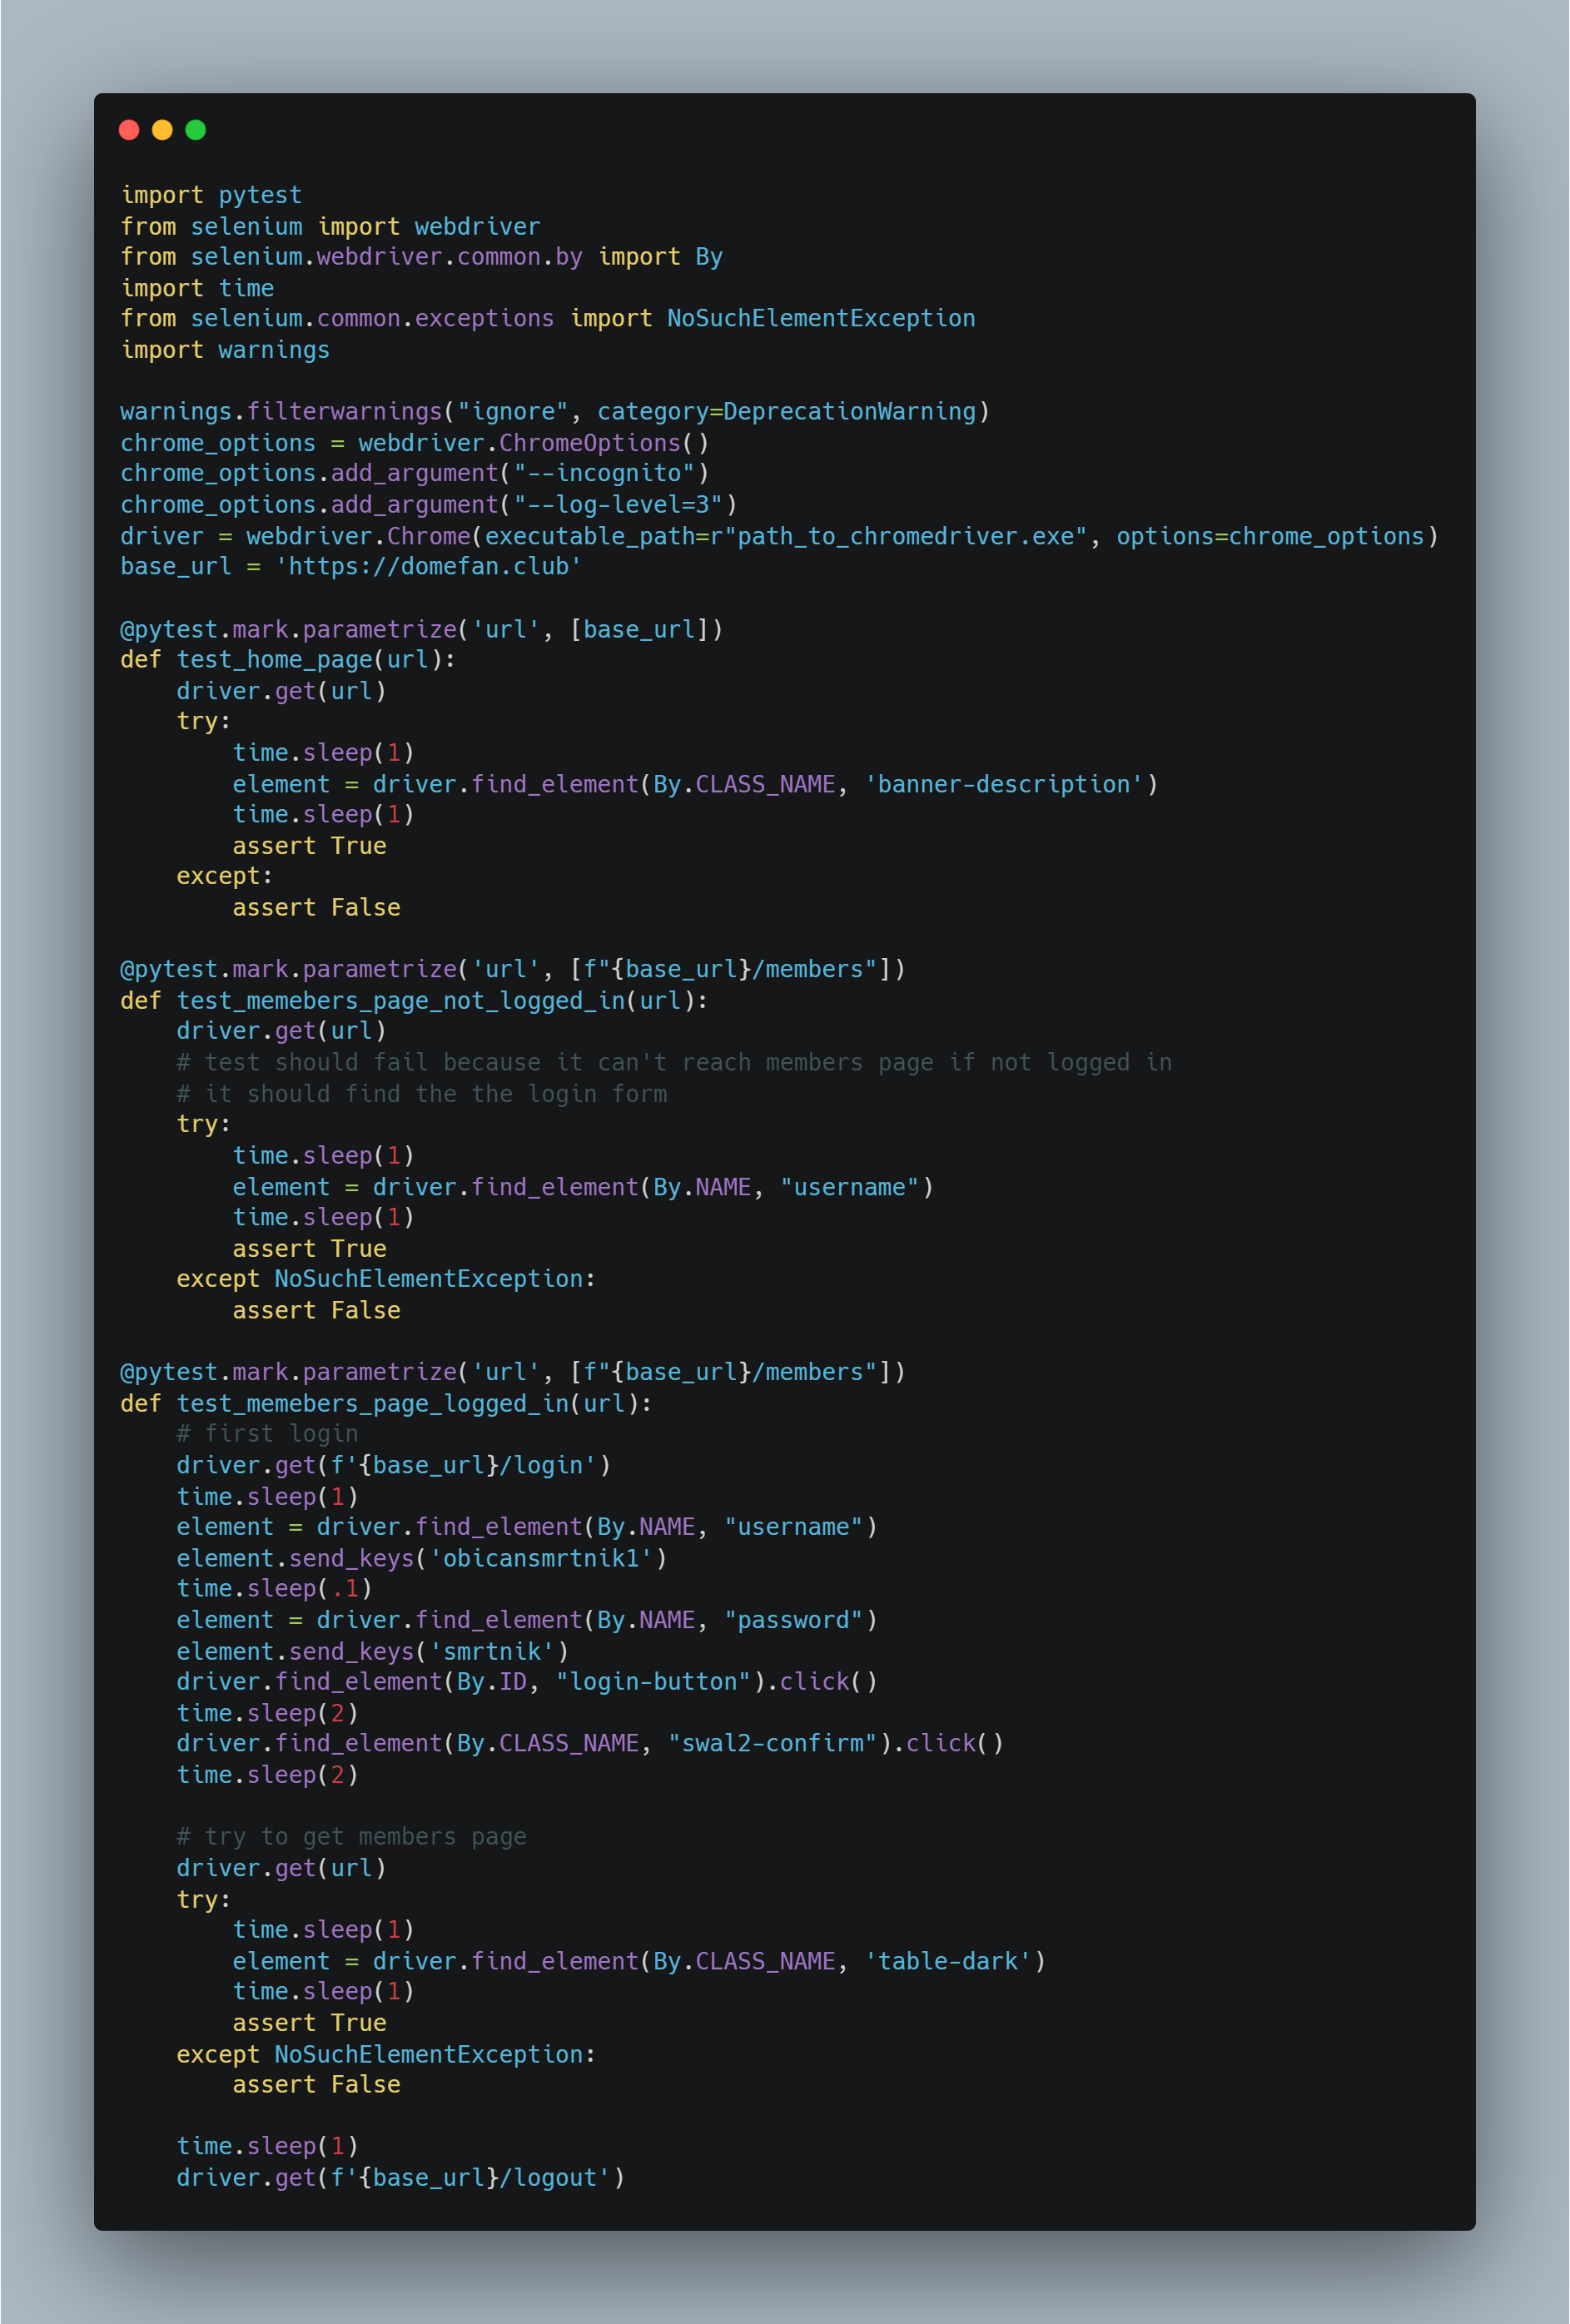
\includegraphics[width=\textwidth]{slike/IspitivanjeSustavaPrviDio.png} %veličina u odnosu na širinu linije
				\caption{Ispitivanje sustava prvi dio}
				\label{fig:IspitivanjeSustavaPrviDio} %label mora biti drugaciji za svaku sliku
			\end{figure}
			\begin{figure}[H]
				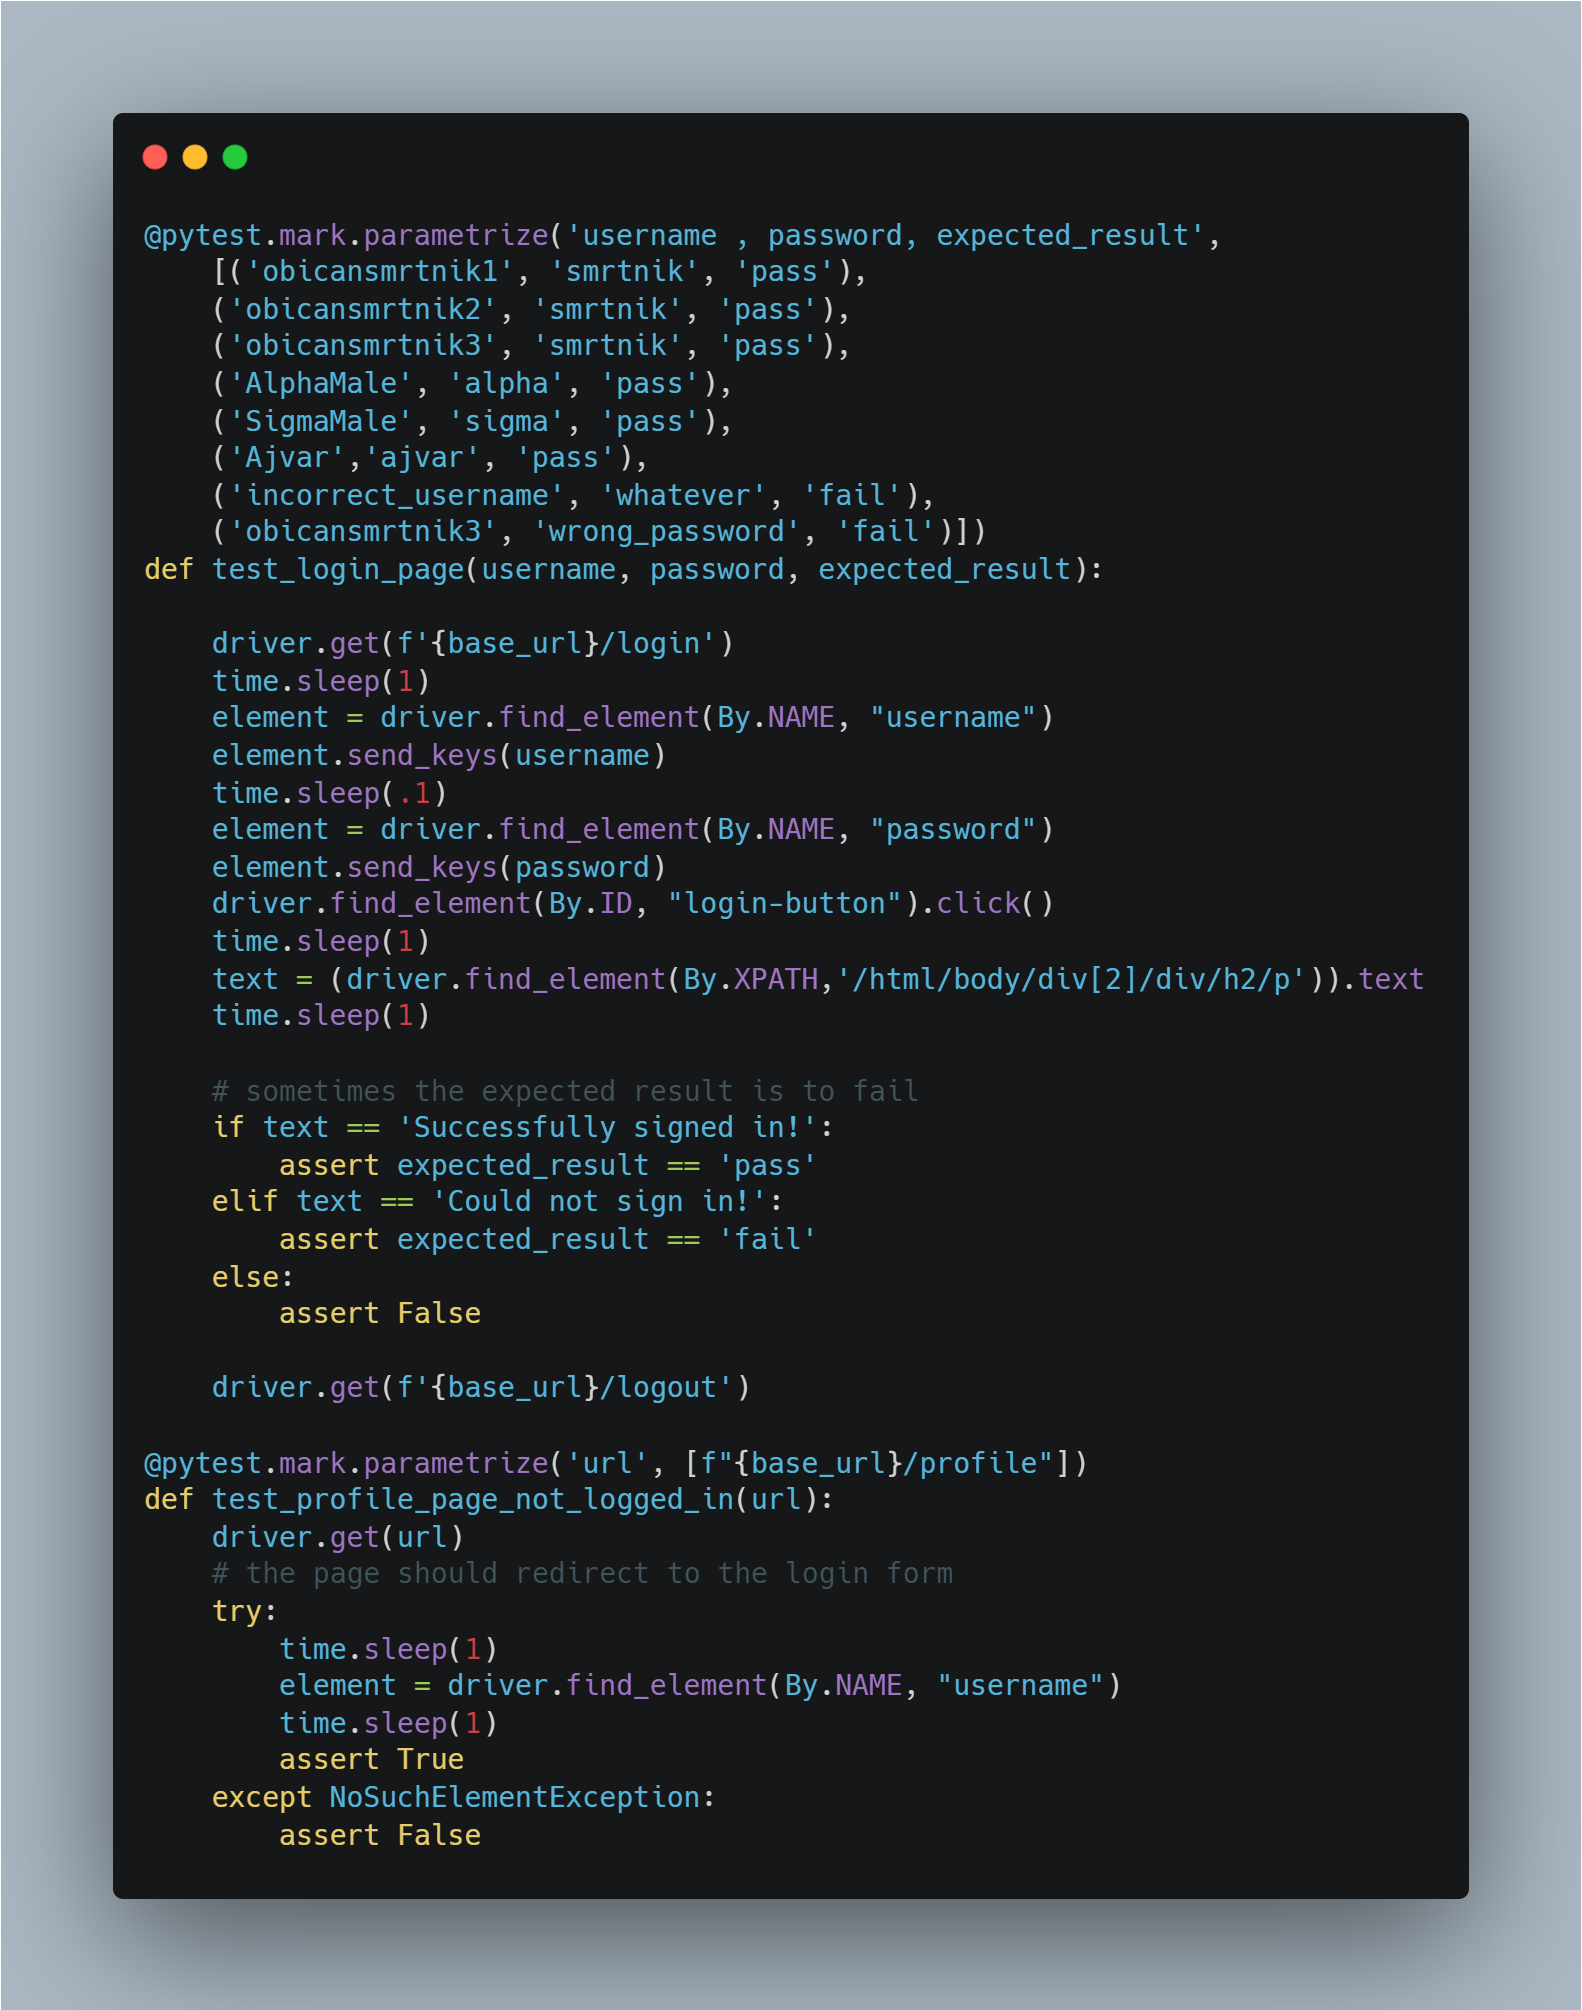
\includegraphics[width=\textwidth]{slike/IspitivanjeSustavaDrugiDio.png} %veličina u odnosu na širinu linije
				\caption{Ispitivanje sustava drugi dio}
				\label{fig:IspitivanjeSustavaDrugiDio} %label mora biti drugaciji za svaku sliku
			\end{figure}
		
			\begin{figure}[H]
				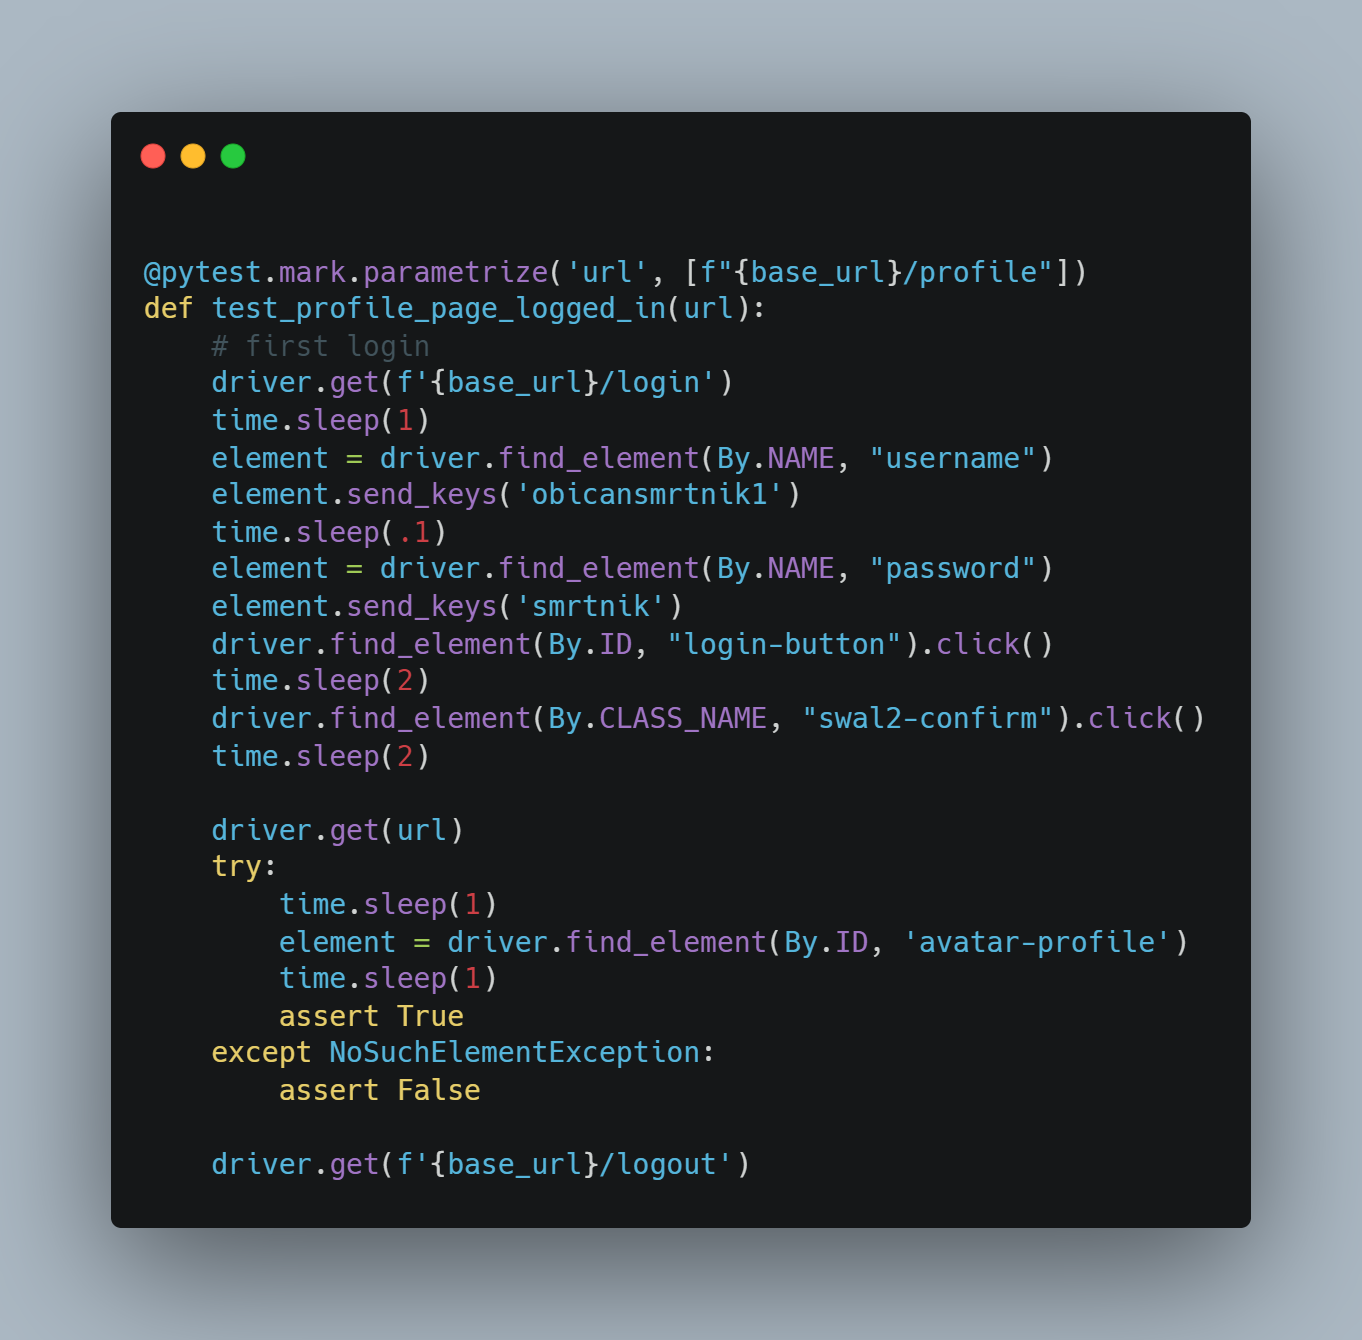
\includegraphics[width=\textwidth]{slike/IspitivanjeSustavaTreciDio.png} %veličina u odnosu na širinu linije
				\caption{Ispitivanje sustava treći dio}
				\label{fig:IspitivanjeSustavaTrećoDio} %label mora biti drugaciji za svaku sliku
			\end{figure}
			
			\begin{figure}[H]
				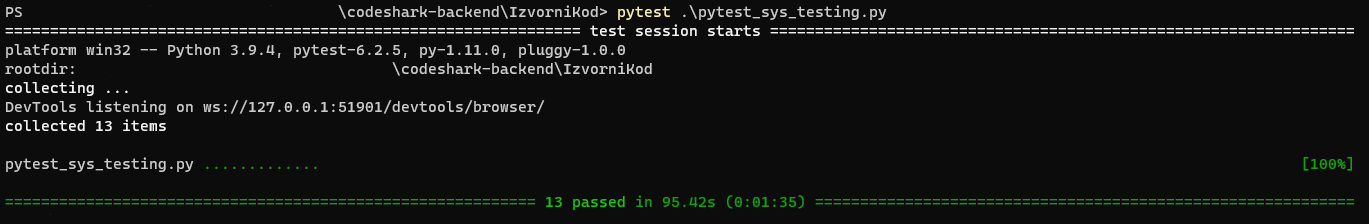
\includegraphics[width=\textwidth]{slike/IspitivanjeSustavaRez.png} %veličina u odnosu na širinu linije
				\caption{Rezultat ispitivanja sustava}
				\label{fig:IspitivanjeSustavaRez} %label mora biti drugaciji za svaku sliku
			\end{figure}
			
			\noindent  \textbf{Rezultat}: \newline
			Svi očekivani rezultati su zadovoljeni.
			 
			 
			
			\eject 
		
		
		\section{Dijagram razmještaja}
			
			Dijagrami razmještaja opisuju topologiju sklopovlja i programsku potporu koja se koristi u implementaciji sustava u njegovom radnom okruženju. Na poslužiteljskom računalu se nalaze web poslužitelj i poslužitelj baze podataka. Klijenti koriste web preglednik kako bi pristupili web aplikaciji. Sustav je baziran na arhitekturi ”klijent – poslužitelj”, a komunikacija između računala korisnika (klijent, zaposlenik, vlasnik, administrator) i poslužitelja odvija se preko HTTPS veze.
			
			
			\begin{figure}[H]
				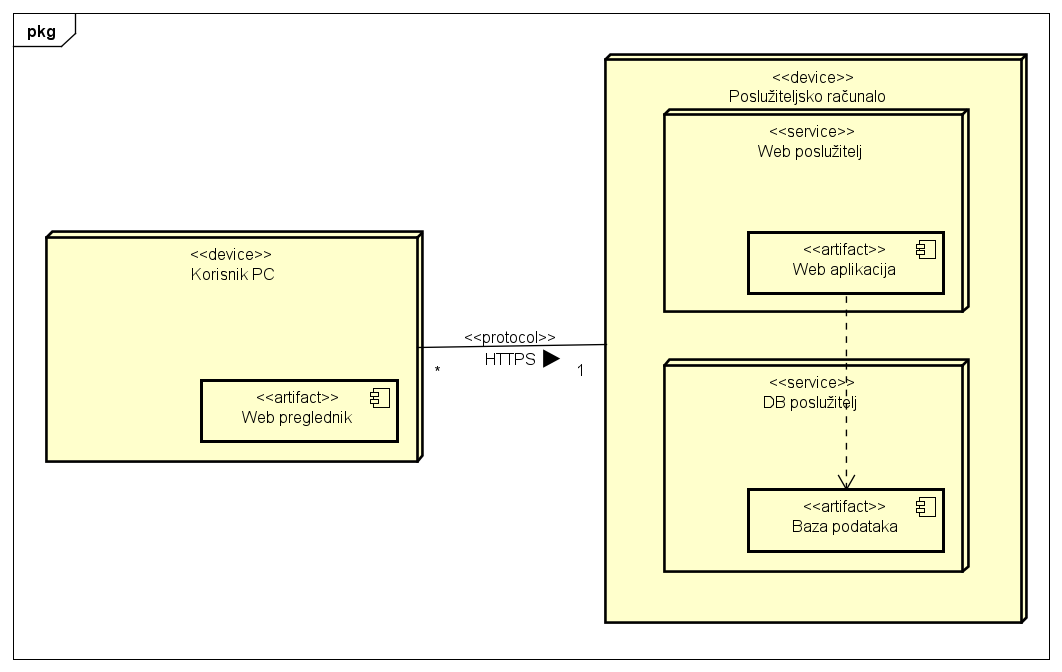
\includegraphics[width=\textwidth]{slike/DijagramRazmjestaja.png} %veličina u odnosu na širinu linije
				\caption{Dijagram Razmještaja}
				\label{fig:DijagramRazmještaja} %label mora biti drugaciji za svaku sliku
			\end{figure}
			
			\eject 
		
		\section{Upute za puštanje u pogon}
		
			\textbf{Instalacija poslužitelja baze podataka}\\
		
			 Potrebno je preuzeti Oracle MySql bazu podataka (za operacijski sustav Windows).
			 Poželjno je skinuti čitav paket Oracle Workbench. Nakon toga je potrebno provesti standardnu instalaciju s postavljanjem korisnika.
			
			
			 \textit{Dovršenu aplikaciju potrebno je pokrenuti na javno dostupnom poslužitelju. Studentima se preporuča korištenje neke od sljedećih besplatnih usluga: \href{https://aws.amazon.com/}{Amazon AWS}, \href{https://azure.microsoft.com/en-us/}{Microsoft Azure} ili \href{https://www.heroku.com/}{Heroku}. Mobilne aplikacije trebaju biti objavljene na F-Droid, Google Play ili Amazon App trgovini.}
			
			
			\eject 